\chapter{Introduction}
\setlist{nosep}

\section{Extragalactic sky}
When looking in a clear night into the sky you can see a whitish band where a lot of stars are located (see figure \ref{fig:milkyway}). 
\begin{figure}[H]
	\centering
		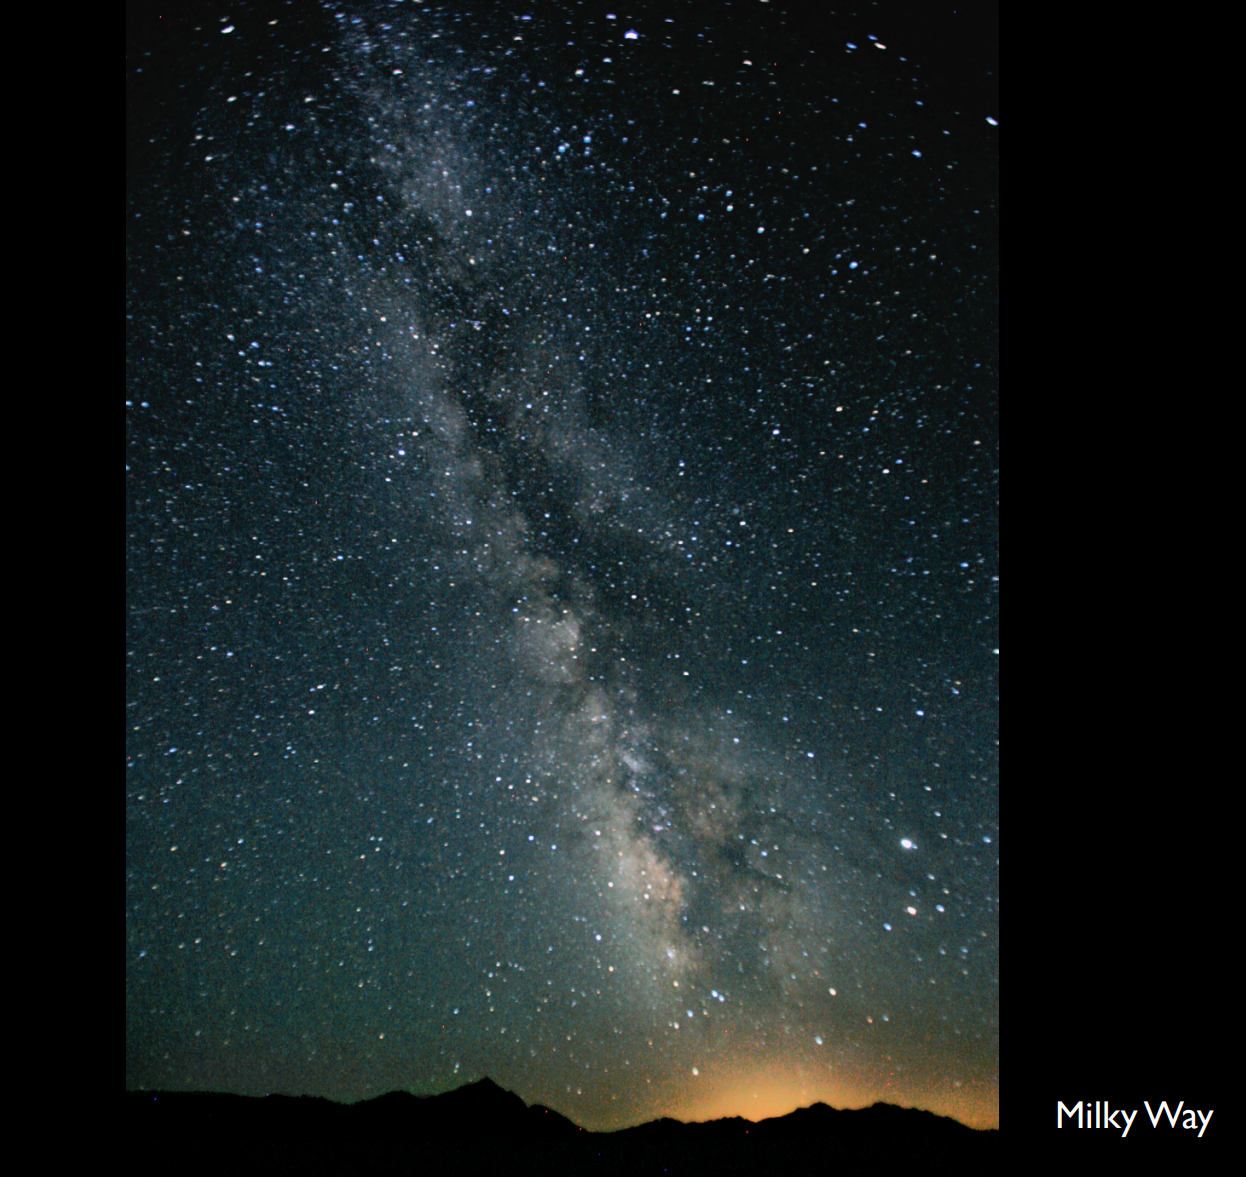
\includegraphics[width=0.9\textwidth]{img/ch-01/milkyway.png}
		\caption{An image of the night sky which shows the milky way.}
		\label{fig:milkyway}
\end{figure}
This band is the milky way the galaxy to which our solar system belongs. If we were able to have a look onto our galaxy from outside of it, we would see something like it is shown in figure \ref{fig:milkywayoutside}. From the image one sees that the milky way has a galactic center which has the form of a bar and spiral arms which come from the center. Our solar system is situated quite far away from the galactic center in one of the arms. 
\begin{figure}[H]
	\centering
		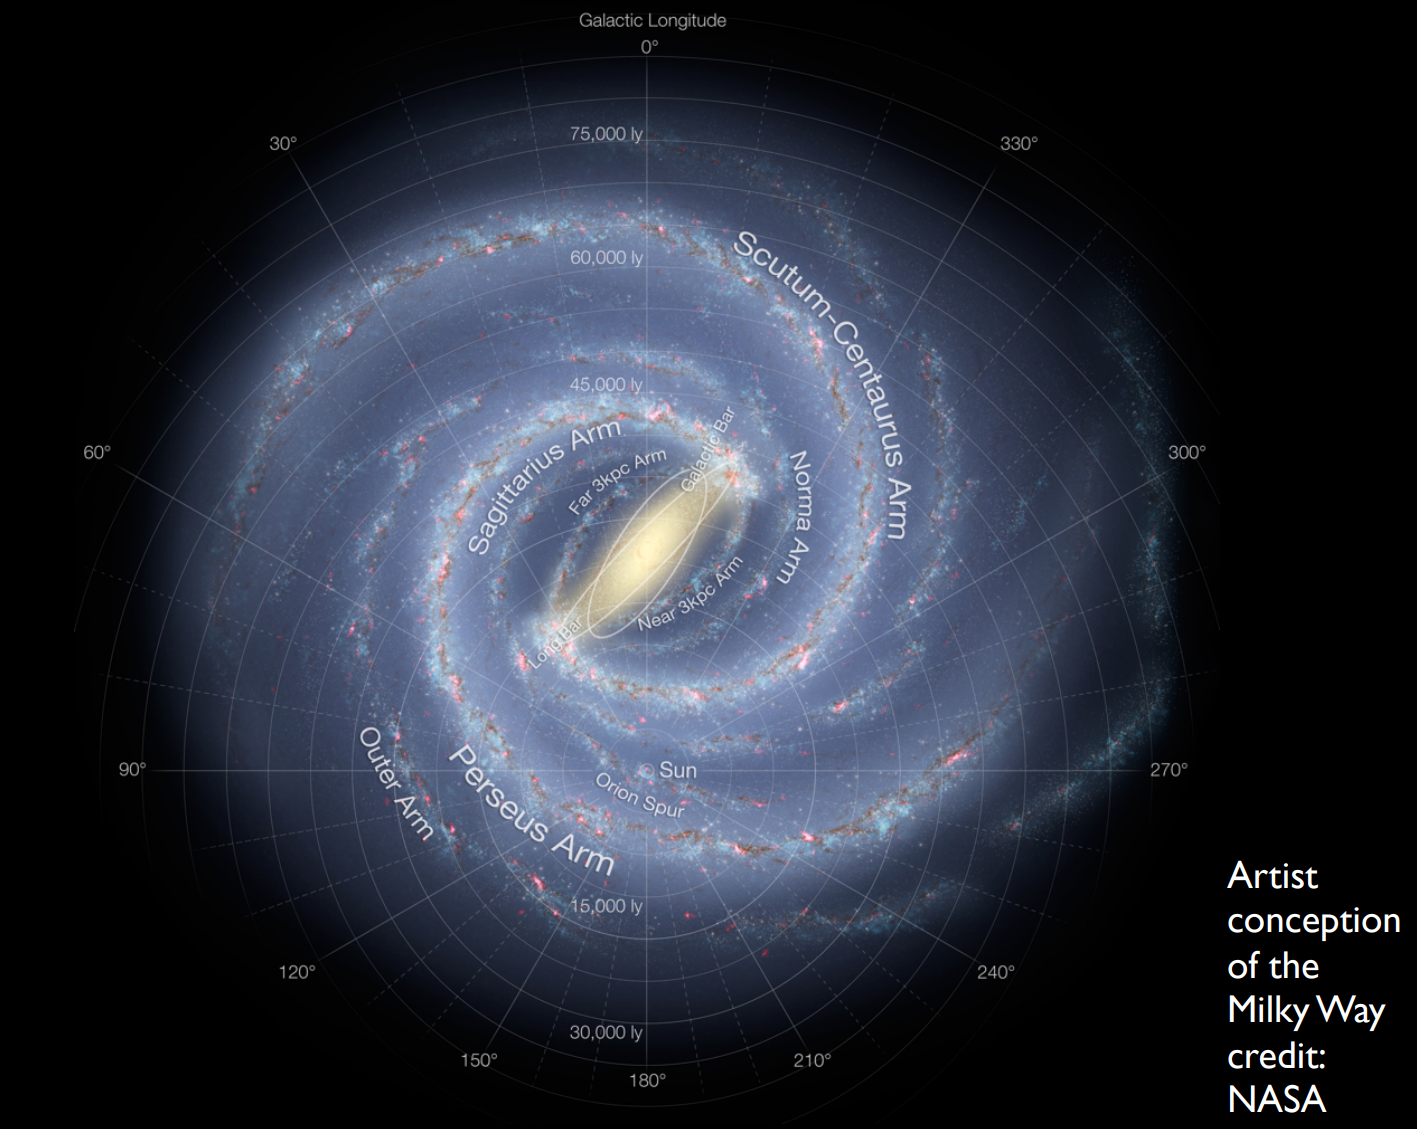
\includegraphics[width=0.9\textwidth]{img/ch-01/milkywayfromoutside.png}
		\caption{An illustration of the milky way showing it from an outside perspective.}
		\label{fig:milkywayoutside}
\end{figure}
But our galaxy is not the only one in our Universe and there are different types of galaxies. The milky way is a so called spiral galaxy. In figure \ref{fig:spiralM101} an other spiral galaxy the M101 is illustrated. A subgroup of spiral galaxies are so called barred spiral galaxies (see figure \ref{fig:barredspiralNGC1300}) they are characterized by the barred shape of their center. Figure \ref{fig:ellipitcalNGC1332} shows an elliptical galaxy and figure \ref{fig:dwarfirregularNGC1427A} is an example for an irregular galaxy, the one shown in the figure is an irregular dwarf galaxy. If a spiral or an irregular galaxy has a really bright galactic center, it is called a Seyfert galaxy (see figure \ref{fig:seyfertNGC1097}). Their are a subgroup of active galactic nuclei and the brightness of the galactic center is probably caused by a super massive black hole in the center of the galaxy. 
\begin{figure}[H]
	\centering
		\begin{subfigure}[b]{0.49\textwidth}
			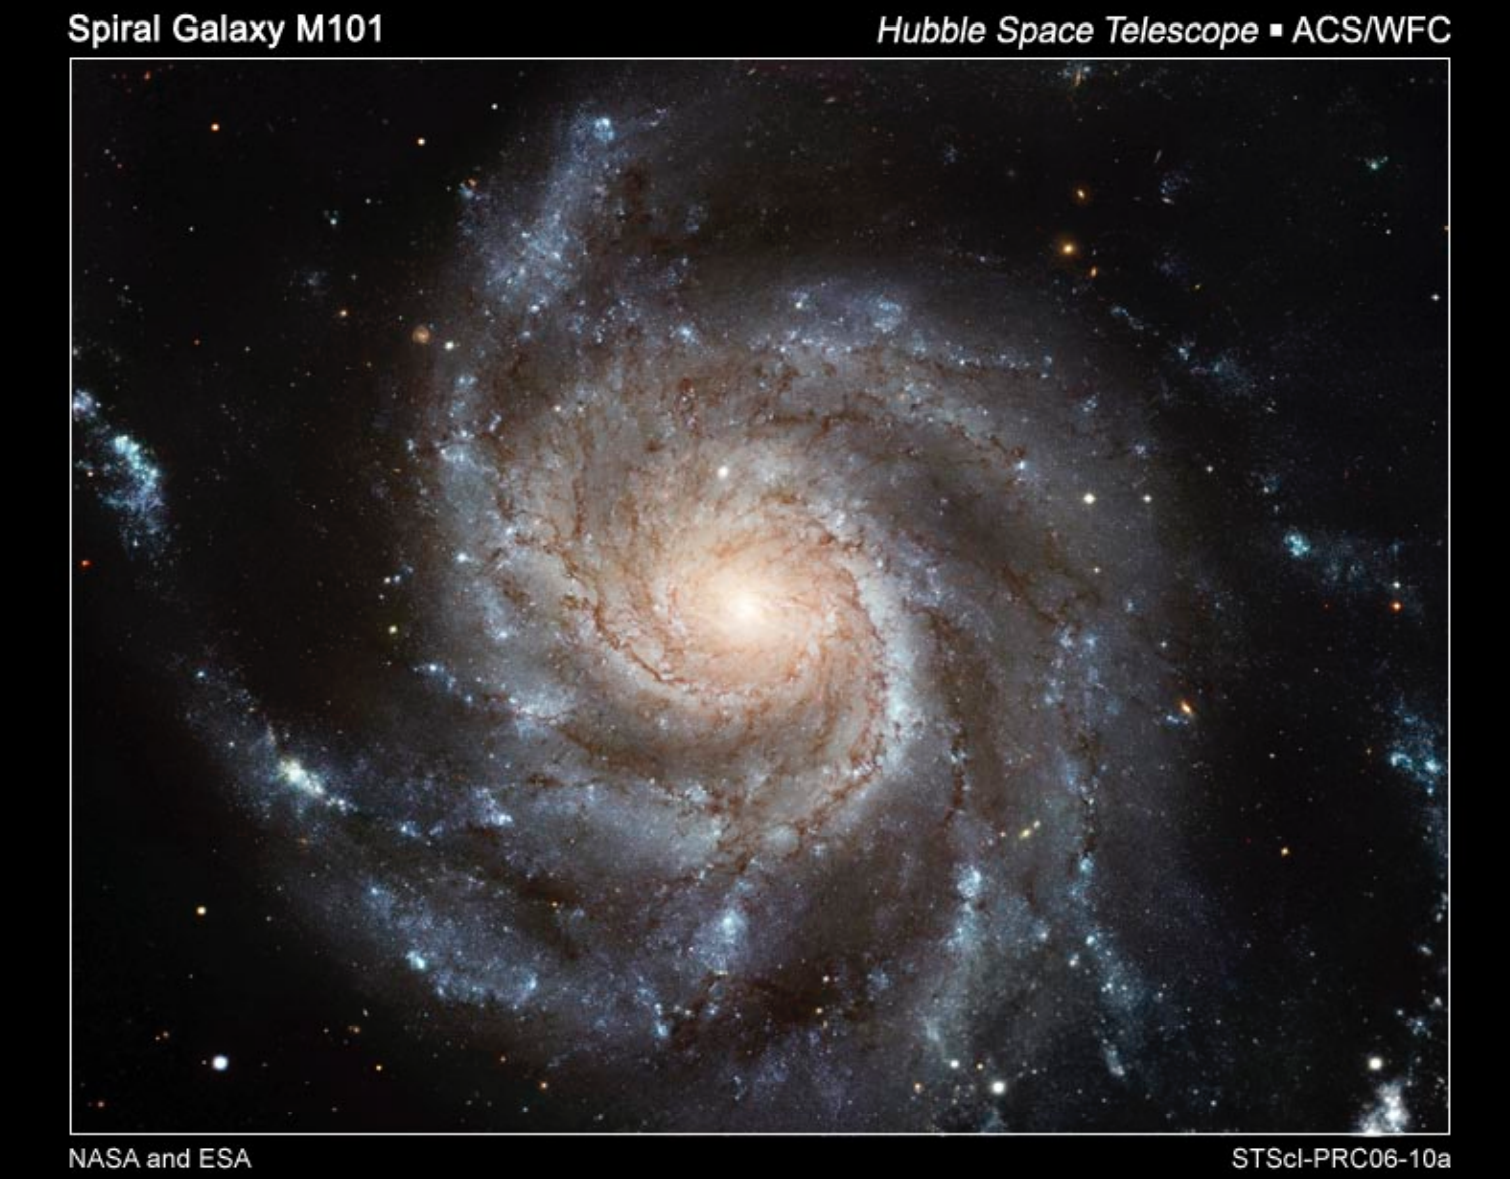
\includegraphics[width=1\linewidth]{img/ch-01/spiralM101.png}
			\caption{}
			\label{fig:spiralM101}
		\end{subfigure}
		\begin{subfigure}[b]{0.49\textwidth}
			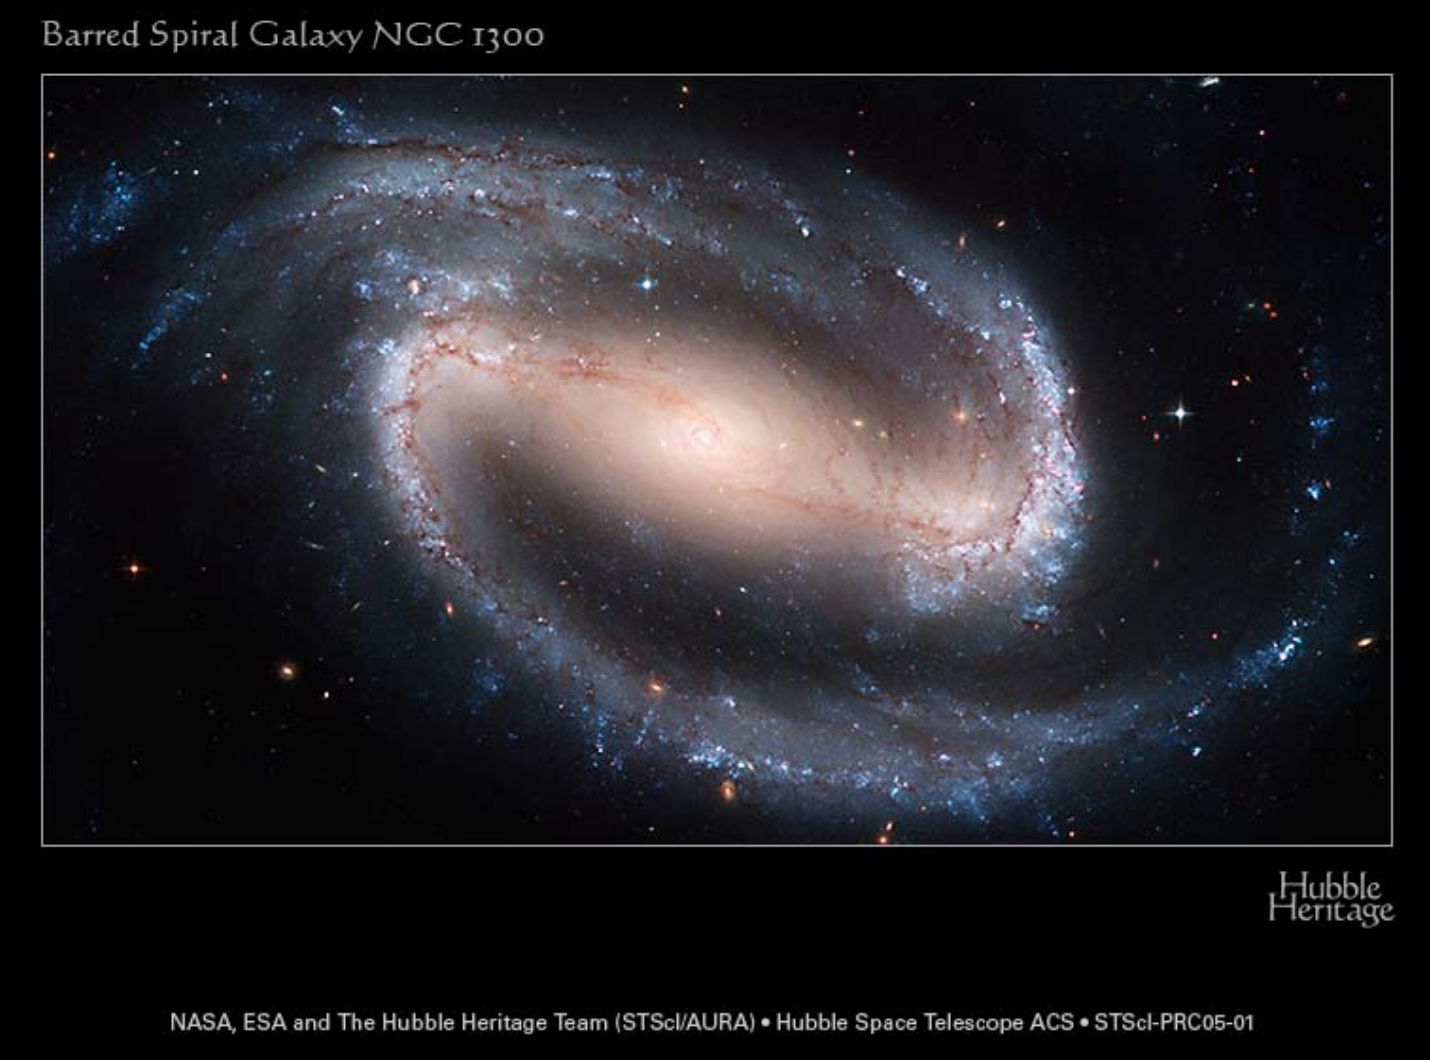
\includegraphics[width=1\linewidth]{img/ch-01/barredspiralNGC1300.png}
			\caption{}
			\label{fig:barredspiralNGC1300}
		\end{subfigure}
		\begin{subfigure}[b]{0.49\textwidth}
			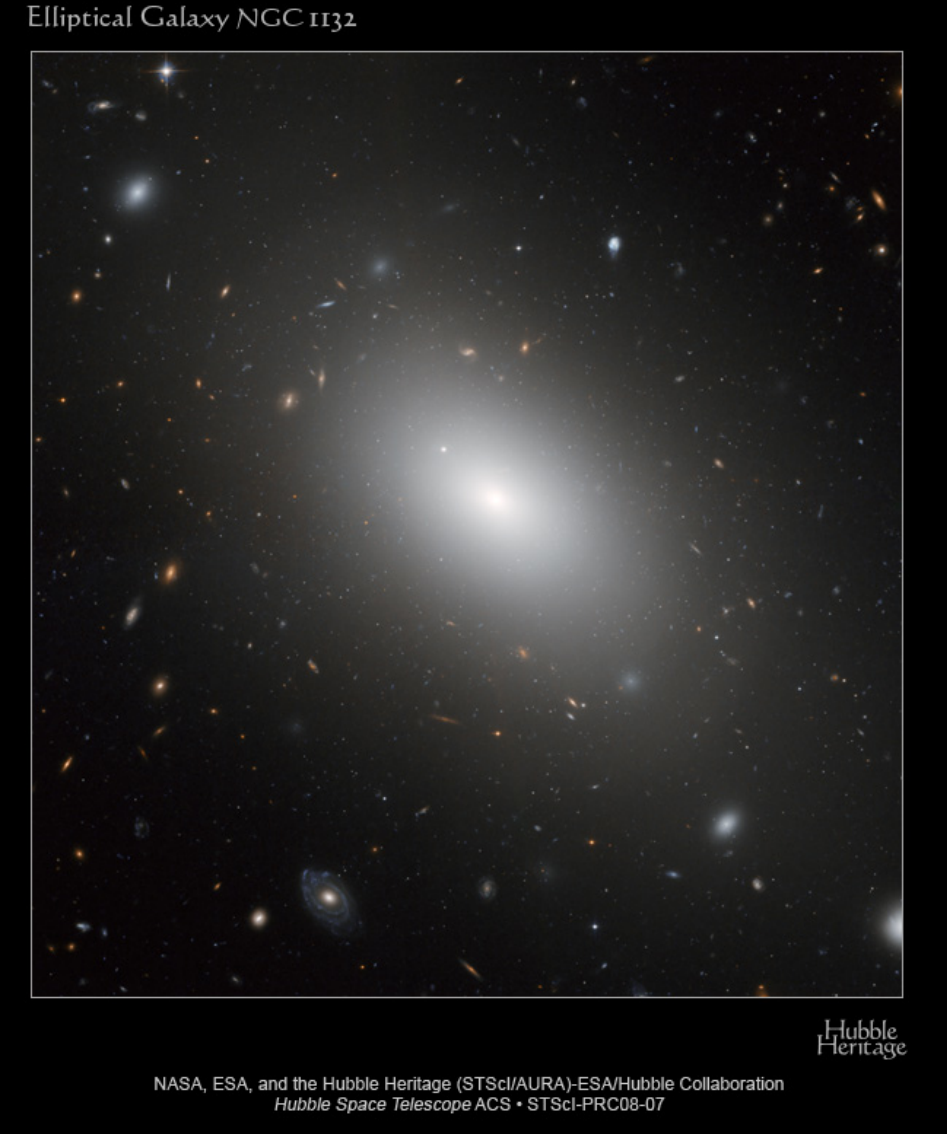
\includegraphics[width=1\linewidth]{img/ch-01/ellipticalNGC1132.png}
			\caption{}
			\label{fig:ellipitcalNGC1332}
		\end{subfigure}
		\begin{subfigure}[b]{0.49\textwidth}
			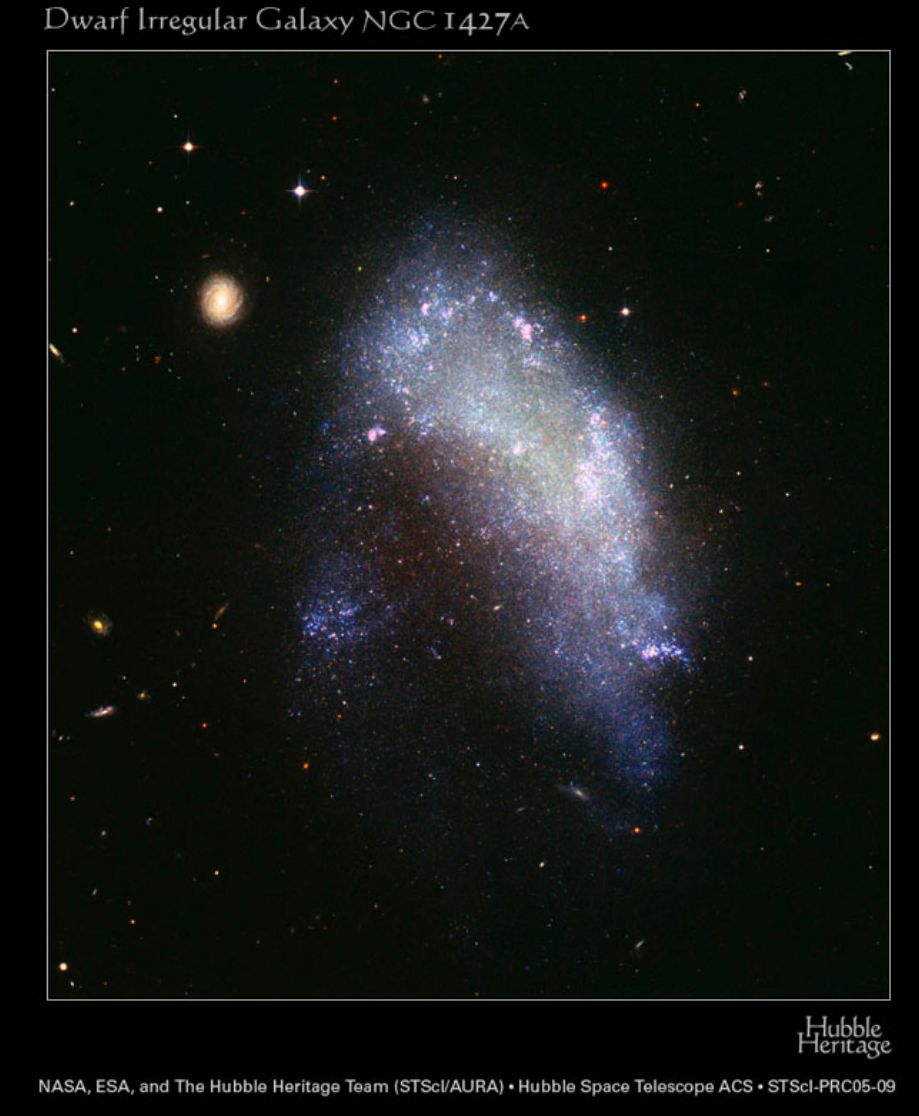
\includegraphics[width=1\linewidth]{img/ch-01/dwarfirregularNGC1427A.png}
			\caption{}
			\label{fig:dwarfirregularNGC1427A}
		\end{subfigure}
		\begin{subfigure}[b]{0.55\textwidth}
			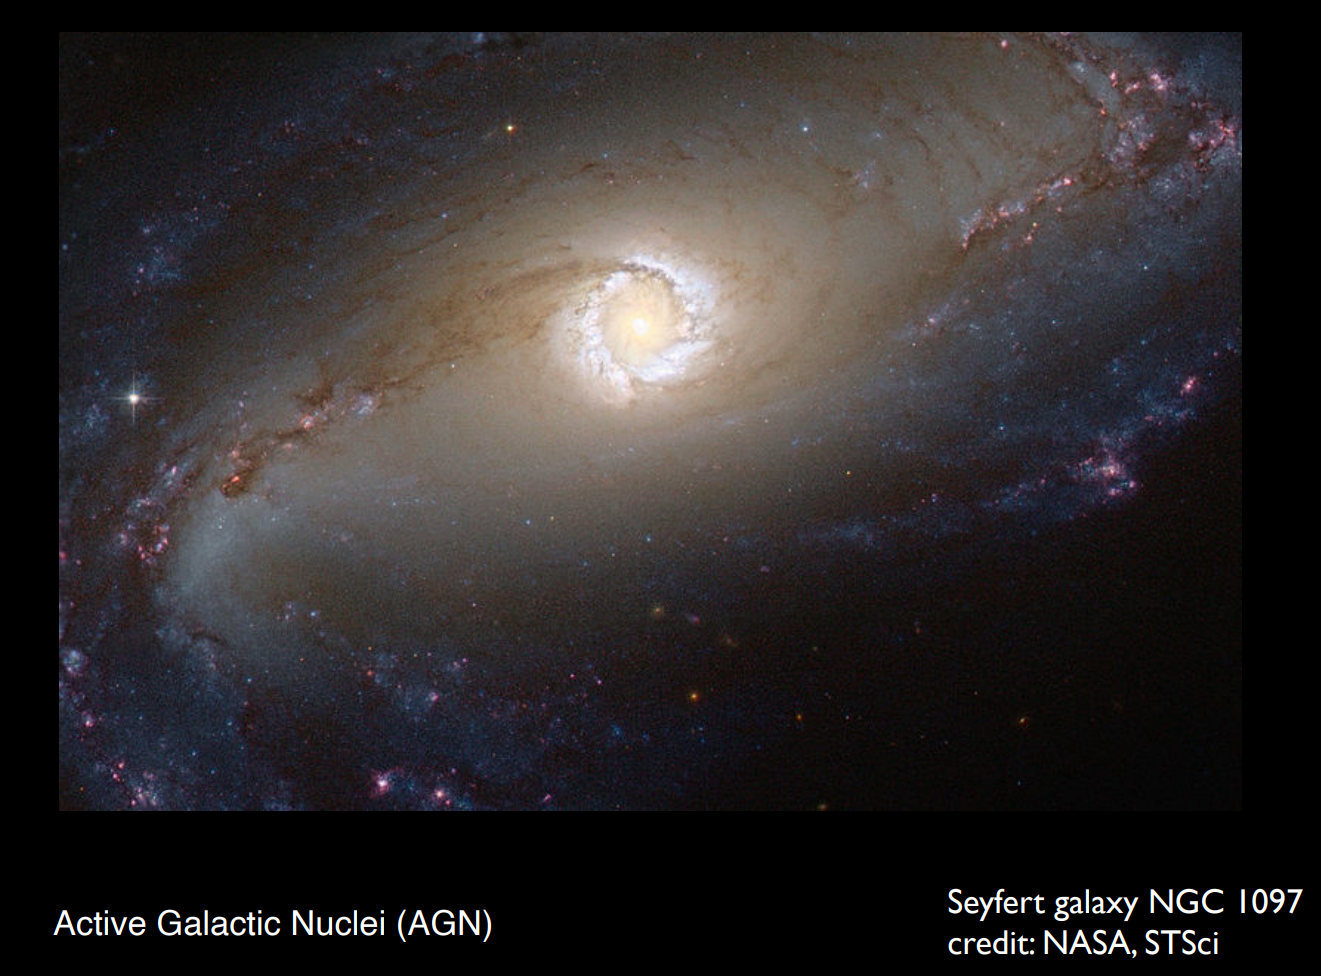
\includegraphics[width=1\linewidth]{img/ch-01/seyfertNGC1097.png}
			\caption{}
			\label{fig:seyfertNGC1097}
		\end{subfigure}
\caption{The images show different types of galaxies: A spiral galaxy (a), a barred spiral galaxy (b), an elliptical galaxy (c), an irregular dwarf galaxy (d) and a seyfert galaxy (e).}
\end{figure}
Galaxies can gather in groups (see figure \ref{fig:galaxygroupHCG16}) or clusters (see figure \ref{fig:galaxyclusterA383}). Galaxy groups do contain up to 50 galaxies and they are the smallest collection of galaxies. Whereas galaxy clusters consist of hundreds to thousands of galaxies. They are the largest gravitationally bound structures in the universe and their mass is around $10^{14}$ - $10^{15}$ solar masses.
\begin{figure}[H]
	\centering
		\begin{subfigure}[b]{0.49\textwidth}
			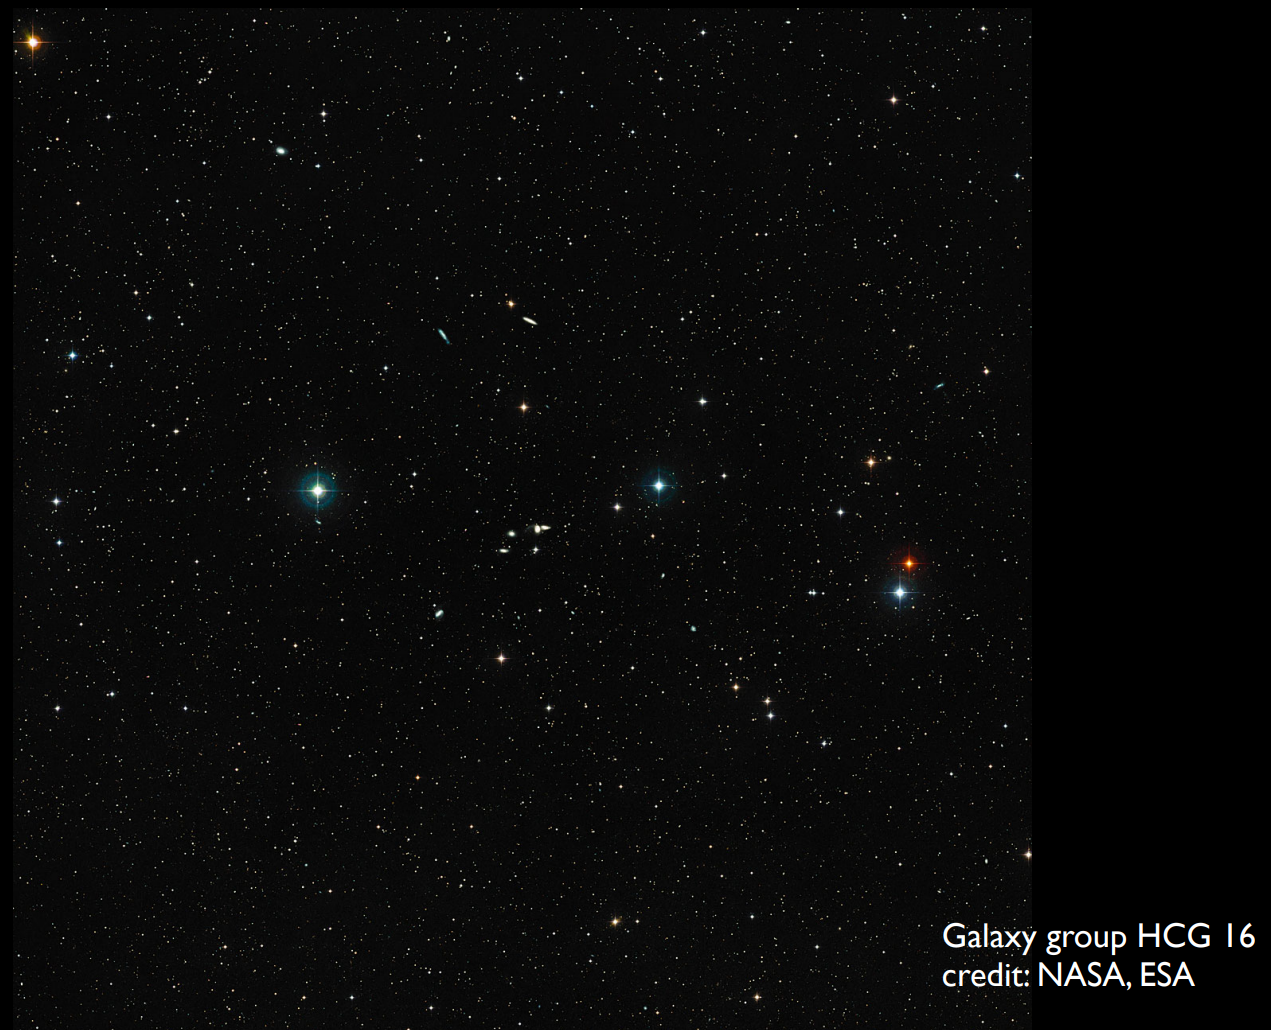
\includegraphics[width=1\linewidth]{img/ch-01/galaxygroupHCG16.png}
			\caption{}
			\label{fig:galaxygroupHCG16}
		\end{subfigure}
		\begin{subfigure}[b]{0.49\textwidth}
			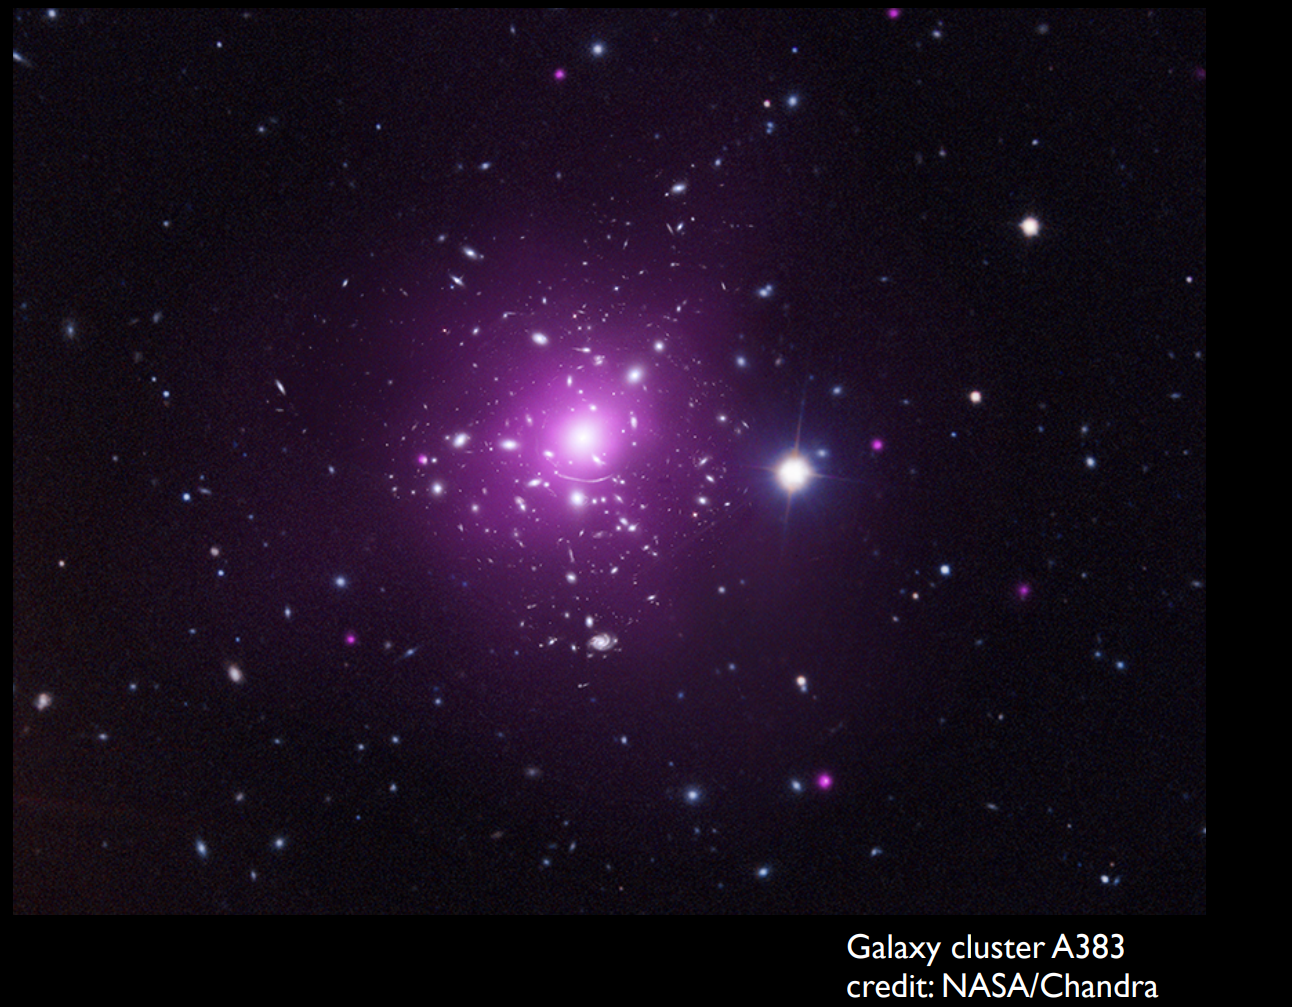
\includegraphics[width=1\linewidth]{img/ch-01/galaxyclusterA383.png}
			\caption{}
			\label{fig:galaxyclusterA383}
		\end{subfigure}
\caption{An example of a galaxy group (a) and of a galaxy cluster (b).}
\end{figure}

\section{Cosmological model}
The standard cosmological model assumes that the universe was initially created in a Big Bang and underwent different epochs until it became the way it is now. Figure \ref{fig:standardcosmologicalmodel} shows the history of the universe, when assuming this model. 
\begin{figure}[H]
	\centering
		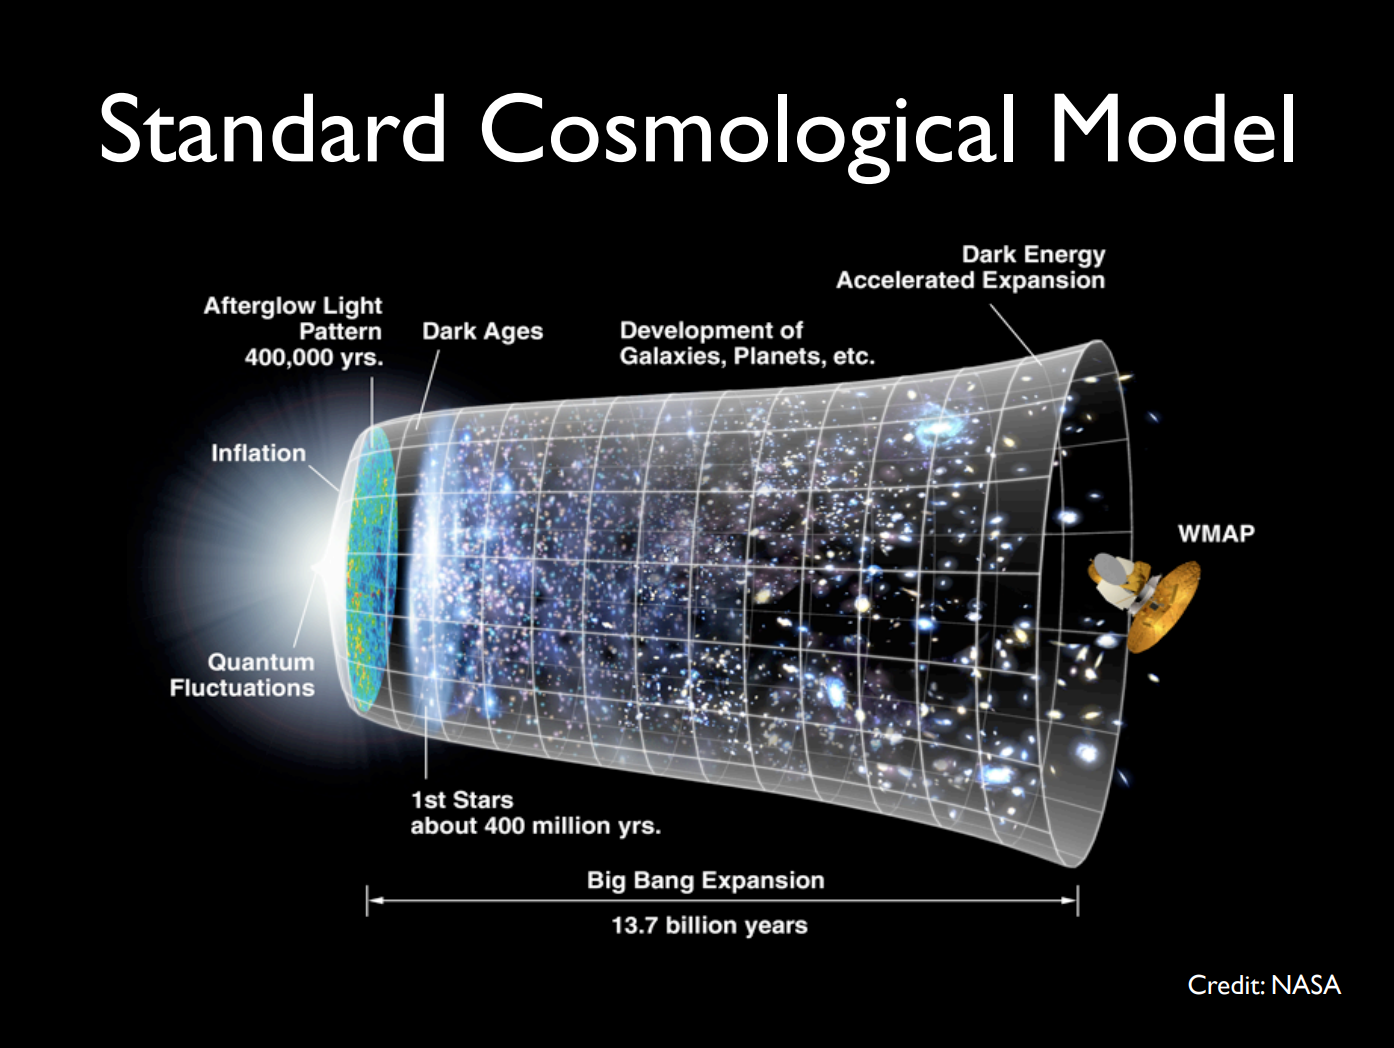
\includegraphics[width=0.7\textwidth]{img/ch-01/standardcosmologicalmodel.png}
		\caption{The standard cosmological model describes the evolution of our Universe starting with the Big Bang.}
		\label{fig:standardcosmologicalmodel}
\end{figure}
From this model we also find that the universe nowadays consist of about 4\% ordinary matter, 20\% dark matter and 76\% dark energy. We will look at this closer in chapter 2. 

\section{Instruments}
For experimental results large telescopes are needed. In order for them to be useful, they have to be placed in places with the right conditions. Therefore, a lot of the telescopes are in space, especially if one wants to observe in the ultraviolet. Figure \ref{fig:electromagneticspectrum} shows the electromagnetic spectrum and at which wavelengths it is necessary to do the observations in space. Radio waves can be observed from earth, for those observation we use array telescopes. 
\begin{figure}[H]
	\centering
		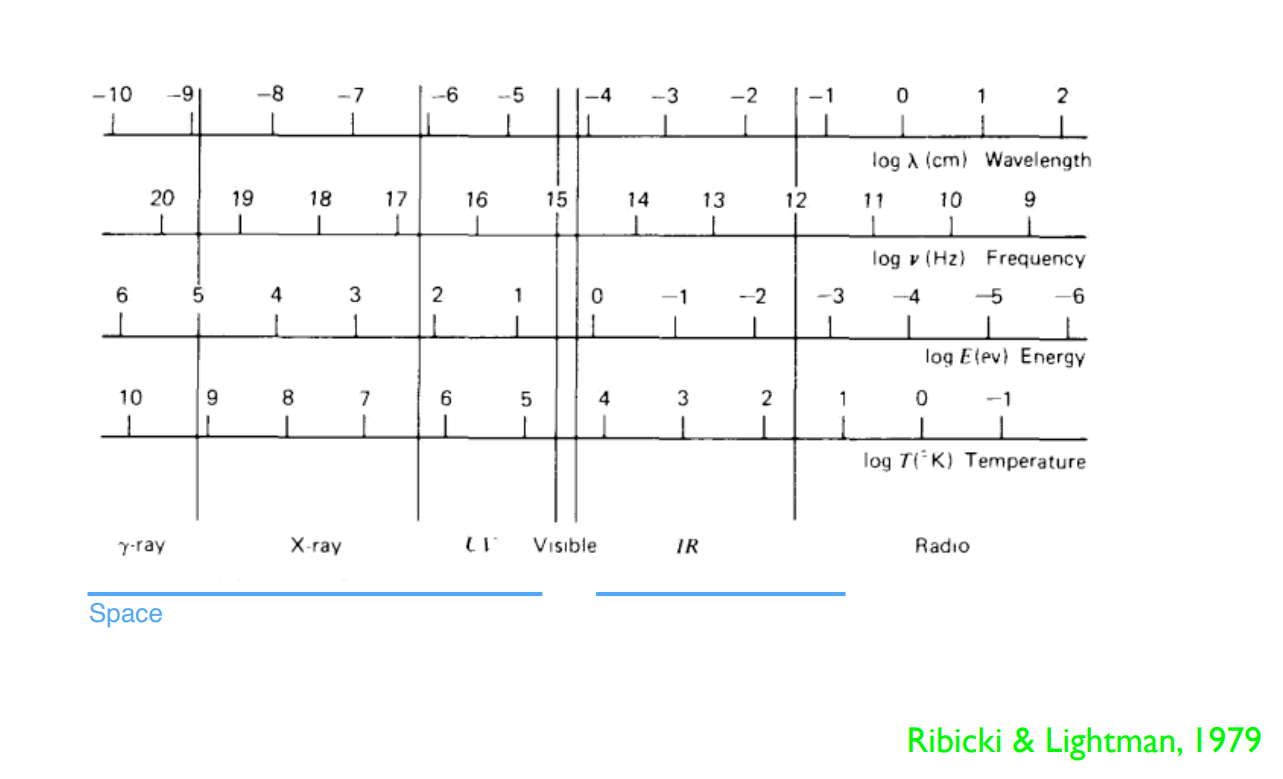
\includegraphics[width=1.0\textwidth]{img/ch-01/electromagneticspectrum.png}
		\caption{The figure shows at which wavelengths it is necessary to put measurement devices in space in order to do observations.}
		\label{fig:electromagneticspectrum}
\end{figure}

\section{Basic concepts}
Astrophysical units are uniquely used in Astrophysics. In order to talk of the mass of different stars, galaxies and more we use the unit of solar masses, where $1 M_{\odot} = 1.99 \cdot 10^{30}$ kg corresponds to the mass of the sun. When talking about time usually years instead of seconds are used, where $1$ yr $ = 3.16 \cdot 10^7$ . Finally we come to the unit of distance. The most known distance scale used in Astrophysics is probably light-years, which is the distance light travels in one year. An other unit for distances which we will use mostly is parsec, $1$ pc $ = 3.09 \cdot 10^{16}$ m $ = 3.26$ ly. Figure \ref{fig:parsec} shows the meaning of a parsec. It is the correlation between the distance between earth and sun and the respective object (a star in the figure) to which we want to know the distance. 1 parsec corresponds to the angle of 1" at the object. 
\begin{figure}[H]
	\centering
		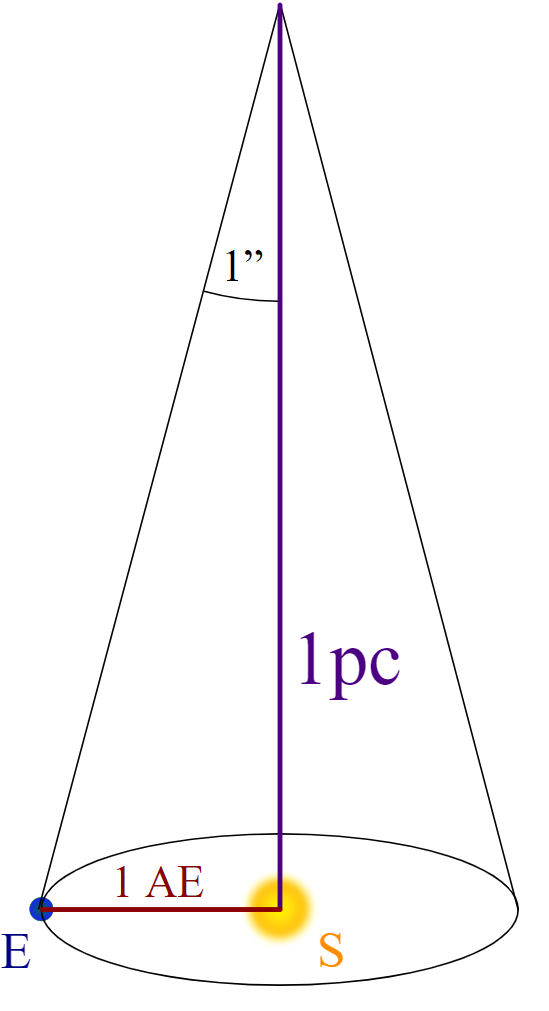
\includegraphics[width=0.3\textwidth]{img/ch-01/parsec.png}
		\caption{One parsec corresponds to the needed distance between sun and object which results into an angle of 1", if one looks at the triangle created by the sun, the object and the earth, which rotates around the sun. \cite{parsec}}
		\label{fig:parsec}
\end{figure}
In order to get a feeling for scales, some mass, distance and time scales are listed here:
\begin{table}[H] 
\label{table:scales}
\centering
\begin{tabular}{|c|c|c|}
\hline
Mass scales & Distance scales & Time scales\\
\hline
Dwarf galaxies $\approx 10^9$ $M_\odot$ & Galaxy size $\approx 10^4$ pc &  Universe age $\approx 14\cdot 10^9$ yr\\
\hline
Galaxies $\approx 10^{12}$ $M_\odot$ & Galaxy cluster size $\approx 10^6$ pc & Sun age $\approx 4.6\cdot 10^9$ yr\\
\hline
Galaxy groups $\approx 10^{13}$ $M_\odot$ & Homogeneity $\approx 10^8$ pc & -\\
\hline
Galaxy clusters $\approx 10^{15}$ $M_\odot$ & Observable Universe $\approx 10^9$ pc & -\\
\hline
\end{tabular}
\end{table}
To talk about stars and other bright objects in the universe we need a way to talk about the luminosity, flux and the magnitude of these objects. The intrinsic luminosity is defined as
\begin{equation}
	L = \frac{energy}{time}
\end{equation}
Whereas the flux at the observer is defined as the luminosity divided by the area. So
\begin{equation}
	F = \frac{L}{4\pi r},
\end{equation}
where r is the distance between object and observer. Usually the flux is with respect to a specific waveband $X$, therefore we write $f_X$. An other possibility to say something about the brightness of the object is the magnitude, which is the most common way. There is the apparent magnitude $m_X$ which describes the brightness of the object seen by the observer (which means here on earth). In order to compare the brightnesses of different objects and to be able to say something about their properties as mass, one needs the absolute magnitude $M_X$. The absolute magnitude is the magnitude one would see at a distance of 10 pc ($r_0 = 10$ pc) to the object. The magnitudes are calculated as follows
\begin{equation}
	m_X = -2.5 \log(f_X/f_{X,0})
\end{equation}
\begin{equation}
	M_X = -2.5 \log(L_X) + C_X
\end{equation}
where $f_{X,0}$ is the flux zero point and $C_X$ is the zero point. For the zero point the star Vega is used, which has a n apparent magnitude of $0$ mag. \\
The relation between the apparent and the absolute magnitude can be used to find the distance $r$ to the object
\begin{equation}
	m_X - M_X = 5\log(r/r_0).
\end{equation}
